%(BEGIN_QUESTION)
% Copyright 2007, Tony R. Kuphaldt, released under the Creative Commons Attribution License (v 1.0)
% This means you may do almost anything with this work of mine, so long as you give me proper credit

Prosesstrenden vist under viser en regulators respons på prosessvariabelsignal og setpunkt. Basert på det du ser i denne trenden, avgjør om regulatoren er direkte- eller reversvirkende, og om den implementerer en reguleringsalgoritme av typen bare P, bare I, eller P+I.

$$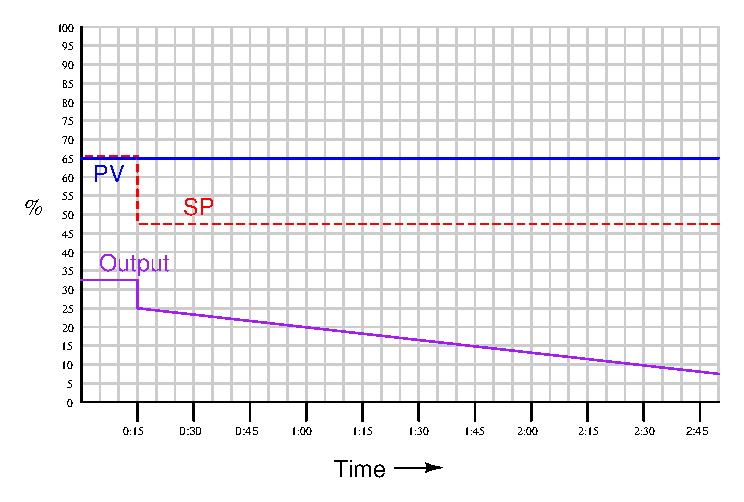
\includegraphics[width=15.5cm]{i01634x01.eps}$$

\vfil

\underbar{file i01634}
\eject
%(END_QUESTION)





%(BEGIN_ANSWER)

Dette er et vurdert spørsmål -- ingen svar eller hint er gitt!

%(END_ANSWER)





%(BEGIN_NOTES)

Dette er en {\bf reversvirkende P+I}-regulator.

\vskip 10pt

Vi kan se at den har ``P''-virkning fordi utgangen trinnendrer seg umiddelbart når SP trinnendres. Vi kan også se at den har ``I''-virkning fordi utgangen ramper når avviket mellom PV og SP vedvarer over tid. Virkemåten er ``revers'' fordi retningen på utgangsendringen er den samme som retningen på SP-endringen (som innebærer at den er motsatt av PV-endringen, siden virkningen av PV- og SP-endringer alltid motvirker hverandre).

%INDEX% Control, proportional + integral: response of real controller to setpoint change

%(END_NOTES)
